\documentclass[12pt,a4paper, xcolor=table]{article}
\usepackage{graphicx}
\usepackage[utf8]{inputenc}
\usepackage{eurosym}
\usepackage[spanish,es-tabla]{babel}
\usepackage[left=2cm, right=2cm, top=2cm, bottom=2cm]{geometry}
\usepackage{afterpage}
\PassOptionsToPackage{hyphens}{url}\usepackage{hyperref}
\usepackage{subfig}
\usepackage[table,xcdraw]{xcolor}

\usepackage{imakeidx}
\newcommand\blankpage{%
    \null
    \thispagestyle{empty}%
    \addtocounter{page}{-1}%
    \newpage}
\renewcommand*\contentsname{Índice: }

\makeindex
\let\olditemize\itemize
\def\itemize{\olditemize\itemsep=0pt}

\begin{document}
\setlength{\parindent}{0pt}
\begin{titlepage}
        \centering
        
\includegraphics[width=0.75\textwidth]{img/logo_uc3m.jpg}\par\vspace{2cm}
        {\huge\bfseries Práctica 2 \\ Análisis de las reseñas de Tripadvisor\par}
        \vspace{0.5cm}
        {\scshape\Large Inteligencia Artificial en las Organizaciones\par}
        \vspace{1.5cm}
        {\scshape\Large Grupo 83-1\par}
        \vspace{1.5cm}
        {\Large\itshape Miguel Gutiérrez Pérez\par}
        {\Large 100383537@alumnos.uc3m.es \par}
        \vspace{1cm}
        {\Large\itshape Mario Lozano Cortés\par}
        {\Large 100383511@alumnos.uc3m.es\par}
        \vspace{1cm}
        {\Large\itshape Alba Reinders Sánchez\par}
        {\Large 100383444@alumnos.uc3m.es\par}
        \vspace{1cm}
        {\Large\itshape Alejandro Valverde Mahou\par}
        {\Large 100383383@alumnos.uc3m.es\par}
        \vspace{5mm}
        {\large GitHub: \textbf{\textit{\href{https://github.com/Pheithar/InteligenciaArtificialOrganizaciones}{InteligenciaArtificialOrganizaciones}}}}
        \vfill

% Bottom of the page
        {\large \today\par}
\end{titlepage}

\tableofcontents

\newpage

\section{Introducción}
    La siguiente sección incluye

\section{Parte 1: Clasificación}
    \subsection{Análisis y preprocesado de datos}
        Explicación de los pasos previos de lo que vimos en clase y división en cat
    \subsection{Experimentación}
        Generalidades de todos los experimentos. hacer hincapié en lo de las stopwords. Caso base
        \subsubsection{Experimentación básica}
        Tablas de cada uno de lo que hicimos esa tarde

        \subsubsection{Experimentación avanzada}
        Combinación de los mejores resultados básicos

    \subsection{Comentario de los resultados obtenidos}
    Mucho text

\section{Parte 2: Clustering}

En la segunda parte de esta práctica se va a realizar una aproximación mediante \textbf{\textit{clustering}}, pero antes de esto, recordar que esta técnica consiste en agrupar instancias sin etiquetar de manera que las instancias pertenecientes aun mismo grupo sean más similares entre sí que con las de otro grupo diferente. 

\vspace{2mm}

En este caso, se agruparán las instancias procesadas que obtuvieron un mejor resultado en la primera parte de la práctica, esta agrupación se hará con el algoritmo \textbf{\textit{K-Medias}}, que se basa en el valor medio de las distancia de cada grupo para generar los grupos. 

\vspace{1mm}

Este proceso se vuelve a realizar en \textit{Weka}, y se compone de los siguientes pasos:

\begin{itemize}
    \item Cargar el archivo \textit{.arff} con los datos generado en la parte anterior.
    \item Generar diferentes modelos a partir de estos datos con \textit{K-Medias} y compararlos.
    \item Analizar el mejor modelo obtenido.
    \item Ejecutar diversos algoritmos de generación de reglas y árboles de decisión con el mejor modelo obtenido.
\end{itemize}


\subsection{Experimentación}

Los experimentos que se llevan a cabo son los que se muestran en la en la Figura X. Los parámetros del algoritmo que se modifican son la \textit{seed} (10, 20 y 30), el \textit{números de clusters} (2, 3, 4, 5 y 6) y el \textit{tipo de distancia} (Euclidea y Manhattan).

\begin{figure}[h]
    \centering
    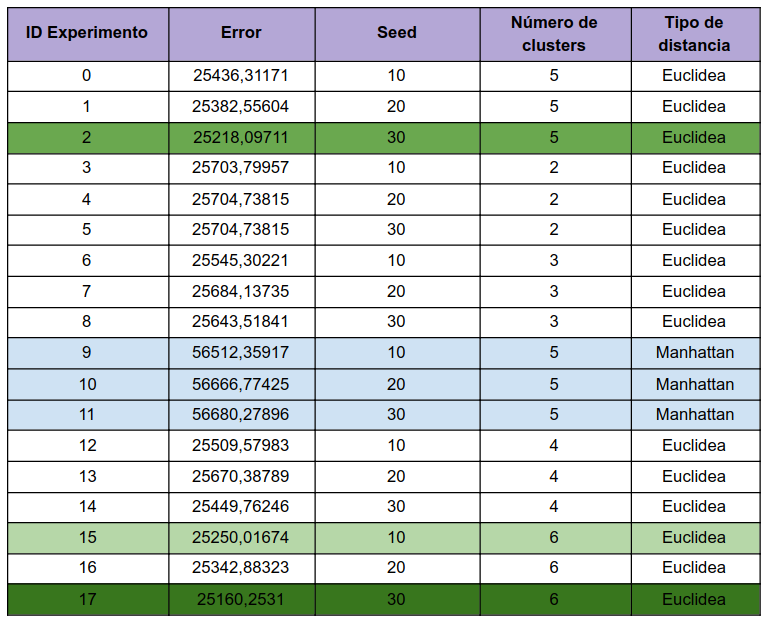
\includegraphics[width=400px]{img/experimentos.png}
    \caption{Tabla de experimentos con \textit{K-Medias}}
    \label{fig:graf_exp1}
\end{figure}


Como se puede apreciar en la Figura X, se prueba para un mismo número de clusters las 3 seeds. Cabe destacar que los experimentos probados con distancia de \textit{Manhattan} cometen mucho más error que los que usan la \textit{Euclidea}. Por este motivo en la gráfica donde se comparan los errores no se añaden, ya que no son relevantes.

\vspace{2mm}

Los errores cometidos por los experimentos que usan distancia \textit{Euclidea} varían en el rango de 25160.25, siendo este el mejor, a 25704.73, siendo este el peor. De estos, los mejores resultados son los marcados en verde.

\vspace{2mm}

Este error representa la suma de las distancias medias a cada cluster, por ello cuanto menor sea el error menor serán estas distancias y como consecuencia las instancias estarán mejor agrupadas.

\vspace{3mm}


A continuación se muestra en la Figura X la gráfica comparativa de los errores para poder visualizar mejor los errores de cada experimento.

\begin{figure}[h]
    \centering
    \includegraphics[width=400px]{img/Comparación errores.png}
    \caption{Gráfica comparativa de los errores}
    \label{fig:graf_exp1}
\end{figure}

Por lo tanto, se concluye con que el mejor resultado es el obtenido en el \textbf{Experimento 17}, así que en la siguiente sección se va a analizar en detalle este modelo.

\newpage


\subsection{Mejor modelo}

El mejor modelo es el obtenido con el Experimento 17, se compone de \textbf{6 clusters} aunque según la gráfica de la Figura X, parece que deja 2 clusters vacíos. Mientras que el cluster 4 es el que tiene mayor número de elementos seguido del cluster 5. Por otro lado los clusters 2 y 3 tienen muchos menos elementos.

\begin{figure}[h]
    \centering
    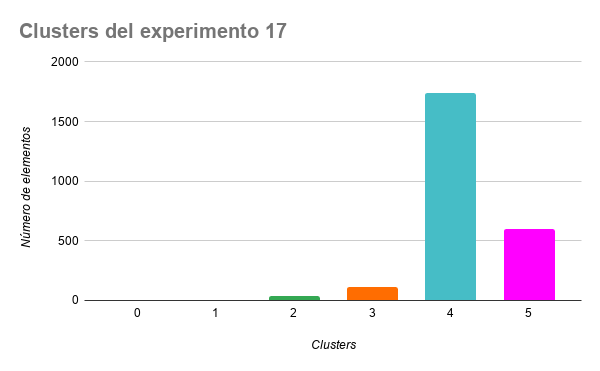
\includegraphics[width=300px]{img/clusters_del_experimento_17.png}
    \caption{Gráfica clusters Experimento 17}
    \label{fig:graf_exp1}
\end{figure}

Ya que con la Figura X no se puede afirmar que los clusters 0 y 1 estén vacíos, se van a visualizar los datos en la siguiente tabla de la Figura X.

\begin{figure}[h]
    \centering
    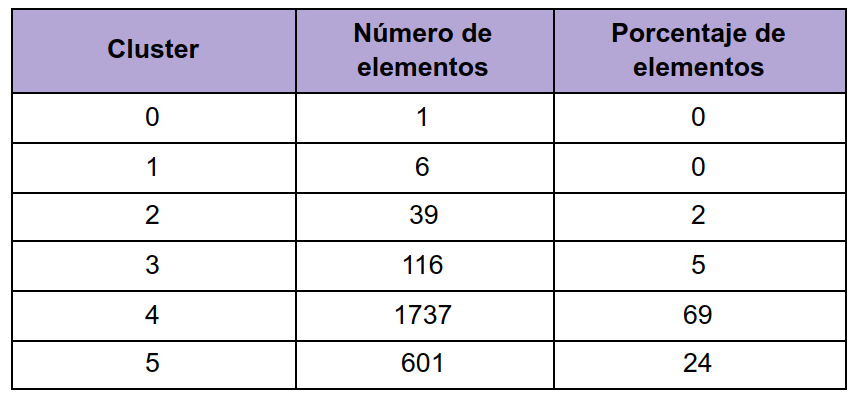
\includegraphics[width=300px]{img/clusters_mejor_exp.png}
    \caption{Tabla clusters Experimento 17}
    \label{fig:graf_exp1}
\end{figure}

\newpage

Una vez que se tienen los números concretos se observa que los cluster 0 y 1 no están vacíos pero poseen muy pocos elementos, 1 y 6 respectivamente. Por lo tanto, se llega a la conclusión de que estos elementos son \textit{outliers} y no aportan nada.

\vspace{4mm}

Tras este análisis del mejor modelo, se ejecutan los siguientes algoritmos de generación de reglas y árboles de decisión con este modelo para descibrir los clusters:

\begin{itemize}
    \item \textit{PART}
    \item \textit{J48}
    \item \textit{RandomForest}
    \item \textit{JRip}
\end{itemize}


\begin{figure}[h]
    \centering
    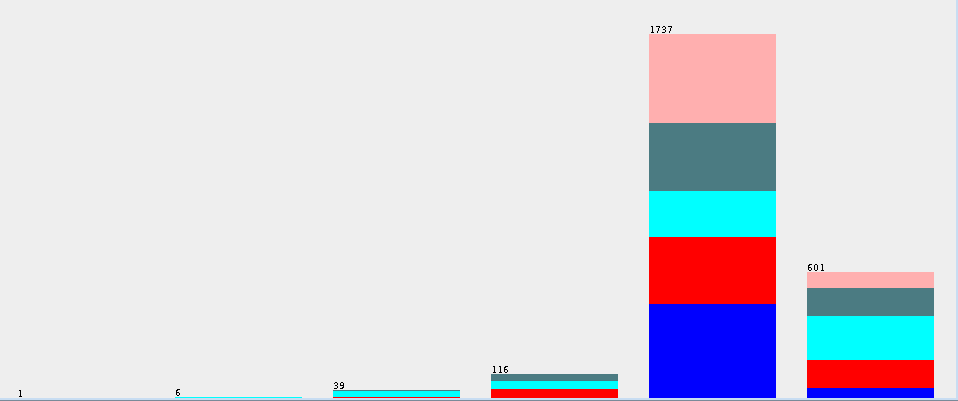
\includegraphics[width=300px]{img/clusters_class.png}
    \caption{Gráfica clusters-clase Experimento 17}
    \label{fig:graf_exp1}
\end{figure}





\section{Conclusiones}

\section{Contexto de la práctica}


\clearpage

\section{Referencias}
    \begin{itemize}
        \item [1.] Introduction to Neurons in Neural Networks. Medium. Consultado en Octubre 2020. Url: \\
        \href{https://medium.com/artificial-neural-networks/introduction-to-neurons-in-neural-networks-71828d040a65}{https://medium.com/artificial-neural-networks}
    \end{itemize}
\printindex



  \section{Anexos}
  \begin{itemize}
    \item [1.] Perceptron Multicapa usando '\textit{K Fold}'\\
    \textbf{\textit{perceptron\_kfold.py}}
    \item [2.] Perceptron Multicapa usando '\textit{split percentage}'\\
    \textbf{\textit{perceptron\_split.py}}
    \item [3.] Programa para realizar la predicción de los modelos\\
    \textbf{\textit{predict.py}}
    \item [4.] Tabla de resultados de los experimentos de la primera parte\\
    \textbf{\textit{valores\_reales\_vs\_predicciones\_\&\_errores\_absolutos\_parte1.xlsx}}
    \item [5.] Tabla de resultados de los experimentos de la segunda parte\\
    \textbf{\textit{valores\_reales\_vs\_predicciones\_\&\_errores\_absolutos\_parte2.xlsx}}
  \end{itemize}


\end{document}
